\section{Results}
\subsection{Individual-model selection does not select a joint distribution}
Table~\ref{tab:marginal} reports the development comparison used to select
individual forecasts. Borg selects the original HGB global arm for pending
tasks (integrated Brier 0.06415) and the relational arm for running tasks
(0.01591). The additional recent-event-count features and the neural
alternatives do not displace these choices. BPI selects the temperature-scaled
three-seed temporal Mixer ensemble (0.09796), ahead of the best HGB candidate
(0.10039). These are development selection results, not an unbiased ranking
on final data.

We now hold each selected CDF fixed across dependence controls.
Table~\ref{tab:main} reports all frozen final models; Figure~\ref{fig:scores}
shows the distinction between count CRPS and reserve loss. The two datasets
are not pooled into a single score. They have different event semantics,
horizons, group structures, and observation spans.
\begin{table*}[t]
\centering\small
\caption{Development integrated Brier used for model selection. Each row selects its calibration variant on development; neural rows average three seeds before scoring. These are selection scores, not final estimates. HGB history is the additional recent-event-count feature arm.}\label{tab:marginal}
\begin{tabular}{lrrr}
\toprule
Individual predictor & Borg pending & Borg running & BPI \\
\midrule
HGB personal & 0.07574 & 0.01599 & 0.10039 \\
HGB global & 0.06415 & 0.01632 & 0.10314 \\
HGB relational & 0.06586 & 0.01591 & 0.10251 \\
HGB history personal & 0.07613 & 0.01600 & -- \\
HGB history global & 0.06900 & 0.01653 & -- \\
HGB history relational & 0.06599 & 0.01609 & -- \\
MIXER ensemble & 0.06928 & 0.01670 & 0.09796 \\
GRU ensemble & 0.06690 & 0.01676 & 0.09871 \\
MLP ensemble & 0.06789 & 0.01792 & 0.10320 \\
\bottomrule
\end{tabular}
\end{table*}

\begin{table*}[t]
\centering\small
\caption{Frozen final evaluation, averaged over forecast origins. Fitted dependence models use three seeds; the historical-residual sampler uses one fixed seed. CRPS and reserve loss are normalized by group size (lower is better); coverage targets 0.9. G: Gaussian; S: common shock. Independent draws are shown for each family to expose Monte Carlo variation. The historical-residual comparator changes aggregate means and lacks entity-level coherence.}\label{tab:main}
\begin{tabular}{lrrrrrr}
\toprule
Model & Borg CRPS & Cov. & Loss$_9$ & BPI CRPS & Cov. & Loss$_9$ \\
\midrule
G: Independent & 0.03417 & 0.659 & 0.1311 & 0.05010 & 0.536 & 0.1177 \\
G: Global & 0.02646 & 0.980 & 0.0551 & 0.04595 & 0.890 & 0.1290 \\
G: Typed static & 0.02587 & 0.906 & 0.0528 & 0.04649 & 0.793 & 0.1222 \\
G: Typed context & 0.02563 & 0.915 & 0.0541 & 0.04630 & 0.828 & 0.1258 \\
G: Permuted incidence & 0.02691 & 0.892 & 0.0586 & 0.04694 & 0.776 & 0.1194 \\
S: Independent & 0.03416 & 0.660 & 0.1310 & 0.05013 & 0.535 & 0.1178 \\
S: Global & 0.02769 & 0.848 & 0.0666 & 0.05095 & 0.579 & 0.1176 \\
S: Typed static & 0.02646 & 0.861 & 0.0639 & 0.05026 & 0.607 & 0.1178 \\
S: Typed context & 0.02611 & 0.866 & 0.0629 & 0.05028 & 0.680 & 0.1179 \\
S: Permuted incidence & 0.02719 & 0.852 & 0.0670 & 0.05003 & 0.593 & 0.1172 \\
Historical residual & 0.03089 & 0.875 & 0.0840 & 0.04387 & 0.831 & 0.1258 \\
\bottomrule
\end{tabular}
\end{table*}

\begin{figure*}[t]
\centering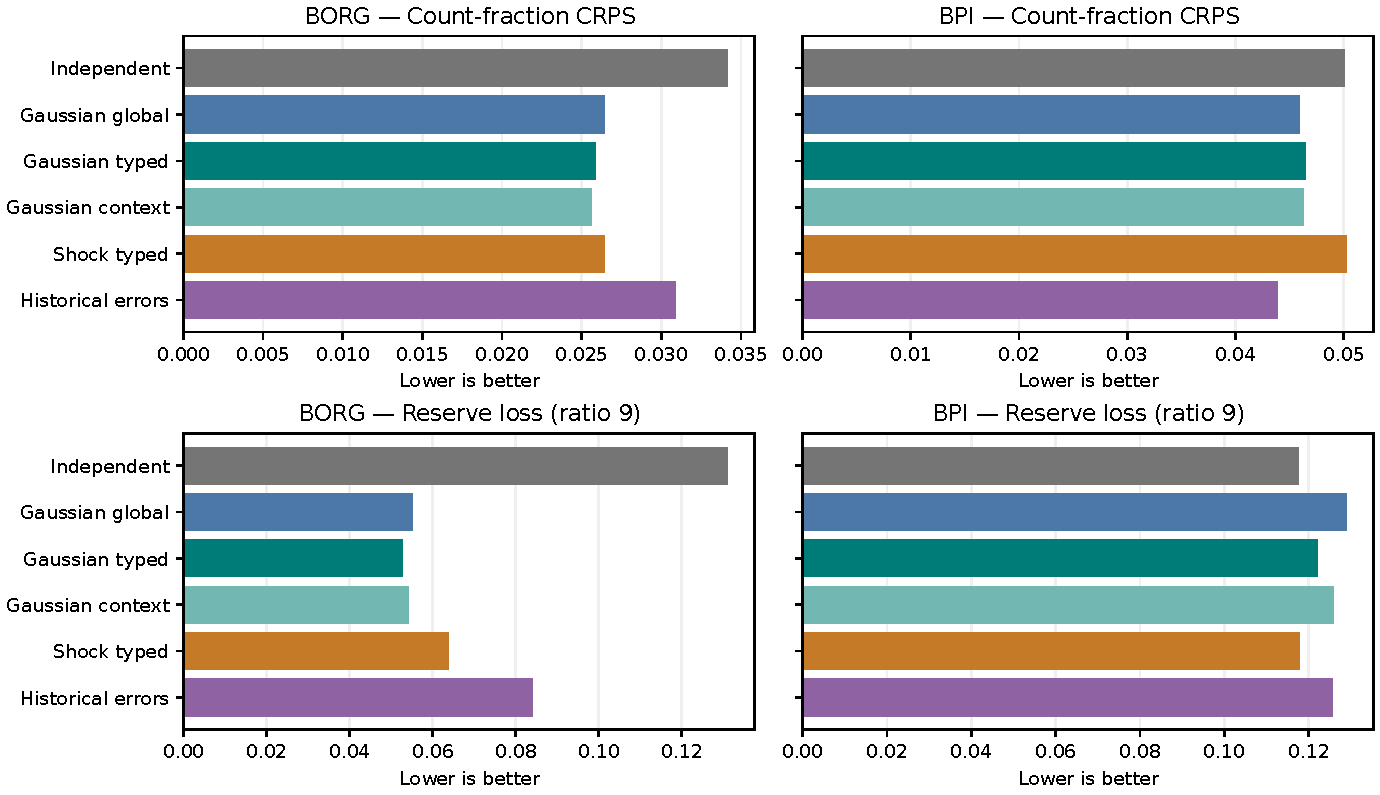
\includegraphics[width=\textwidth]{figures/joint_scores.pdf}
\caption{Final count-fraction CRPS and reserve loss for representative controls.
The same individual CDFs underlie the Gaussian and common-shock comparisons.
Historical errors are a separate direct aggregate forecast. Lower values are
better on each axis; the two axes measure different objectives.}
\label{fig:scores}
\end{figure*}
\subsection{Cluster: shared variation matters, with an additional relation signal}
Across 28 final cluster origins, the development-selected Gaussian static
model reduces macro count-fraction CRPS from 0.03417 to 0.02587, a 24.3\%
improvement over independent sampling. The mean paired difference is
$-0.00829$, with a one-day block interval $[-0.01056,-0.00611]$ and a two-day
interval $[-0.00985,-0.00686]$. At reserve penalty ratio 9, loss falls from
0.13106 to 0.05280, a 59.7\% reduction in this declared proxy. Its paired
one-day interval is $[-0.11744,-0.04280]$ for a mean difference of $-0.07826$.
These are within-trace estimates over seven final days, not independent-task
confidence bounds or measured deployment savings.

Most of the CRPS gain already appears with a global factor: its score is
0.02646. Adding typed relation factors improves that by a further 2.2\%, with
paired difference $-0.000583$ and one-day interval
$[-0.001043,-0.000185]$. At ratio 9, the corresponding global-to-static loss
change is 0.05506 to 0.05280. The large independent-to-static improvement
therefore must not be attributed entirely to graph relations.

The incidence control localizes the additional relation signal. Permuting
memberships increases static-model CRPS from 0.02587 to 0.02691. The paired
difference for true minus permuted incidence is $-0.001031$, with one-day
interval $[-0.001175,-0.000873]$. Job-level CRPS changes most: 0.01451 with
true incidence versus 0.01729 with permuted incidence. Machine-level CRPS
changes from 0.02504 to 0.02535; population CRPS is essentially unchanged
(0.03807 versus 0.03808). Under this controlled sampler intervention, correct
job grouping carries predictive information beyond individual event risk and
global random variation.

Macro coverage requires a qualification. Static Gaussian coverage averages
0.906 across projections, compared with 0.659 for independence. However,
static population coverage is only 0.763, while job and machine coverage are
0.978 and 0.976. Its near-nominal macro value therefore does not establish
calibration within every projection. Independence is particularly unreliable
for the population count, with coverage 0.100. This projection breakdown is
more informative than a single aggregate coverage number.

The context model obtains a slightly lower mean CRPS, 0.02563, but its
context-minus-static difference has one-day interval
$[-0.000661,0.000195]$. Its reserve loss is also slightly higher, 0.05413.
The evidence does not establish a consistent benefit from the additional
context network. Common-shock static factors improve over their independent
control (0.02646 versus 0.03416), but are weaker than Gaussian static factors
on the principal mean scores. The historical-residual comparator has CRPS
0.03089 and reserve loss 0.08400. It is useful as an aggregate-error baseline,
but it does not explain away the selected model's cluster improvement.

\subsection{Workflow: distributional improvement and decision loss diverge}
On the 61 frozen final workflow origins, the development-selected Gaussian
global model reduces macro count-fraction CRPS from 0.05010 to 0.04595, an
8.3\% improvement over independent sampling. Its mean paired difference is
$-0.00415$; the 14-day block interval is $[-0.00638,-0.00188]$, and the 28-day
interval also excludes zero. Mean 90\% coverage rises from 0.536 to 0.890,
while normalized interval width rises from 0.140 to 0.222. This illustrates a
practical failure of independent sampling: reasonable individual probabilities
can induce overly concentrated collective forecasts.

The projection breakdown localizes the effect. Population CRPS improves from
0.03421 to 0.02728 and population coverage from 0.219 to 0.869. Handler-group
CRPS improves more modestly, from 0.06599 to 0.06462, with coverage rising from
0.853 to 0.911. Equal projection weighting keeps these effects visible rather
than allowing the many handler groups to obscure the population result.

That improvement does not extend to the specified reserve loss. At under/over
ratio 9, the selected model's loss is 0.12899 versus 0.11770 for independence,
a 9.6\% increase. The paired difference is 0.01129; its 14-day block interval
is $[-0.00117,0.02129]$, while the 28-day interval is $[0.00426,0.01746]$.
The direction of the mean tradeoff is clear, but its uncertainty depends on
the block choice. We therefore report it as a held-out decision-loss tradeoff,
not a universally established cost penalty. At ratio 3, the mean loss likewise
increases, from 0.08933 to 0.09873.

Observed handler incidence provides a smaller, distinct signal. Gaussian
static factors obtain CRPS 0.04649, compared with 0.04694 after risk-stratified
incidence permutation. The difference, $-0.000454$, has a 14-day block interval
$[-0.000726,-0.000188]$. However, the corresponding reserve loss increases
from 0.11936 under permutation to 0.12219 under true incidence; the paired
interval for this increase is $[0.00119,0.00442]$. Thus, even the same
relation-incidence control can favor one model under a distributional score
and the other under a decision loss. It does not identify a causal effect of
actual handler assignment.

The richer context model does not establish a reliable improvement over the
static model: its mean CRPS difference is $-0.000188$, with a 14-day interval
$[-0.000626,0.000262]$. The common-shock static model has CRPS 0.05026 versus
0.05013 for its independent control. Merely adding a dependence model is
therefore insufficient, and the choice of family matters.

The direct historical-residual comparator achieves the lowest aggregate CRPS
among these workflow comparisons, 0.04387, while its coverage is 0.831 and its
ratio-9 loss is 0.12576. It can shift aggregate means and is not a
matched-marginal ablation. Its mean CRPS advantage over the selected Gaussian
model is not resolved by the block intervals: the Gaussian-minus-residual
difference is 0.00208, with a 14-day interval $[-0.00070,0.00536]$.
This distinction is consequential: at 14 days, the
selected individual ensemble predicts an average population resolution
fraction of 0.5252 versus the observed 0.5792. Every matched-marginal copula
inherits that mean bias. The residual baseline's advantage is evidence for
retaining simple aggregate-error controls, rather than evidence that its
separately sampled projections form a better entity-level joint law.

\begin{figure*}[t]
\centering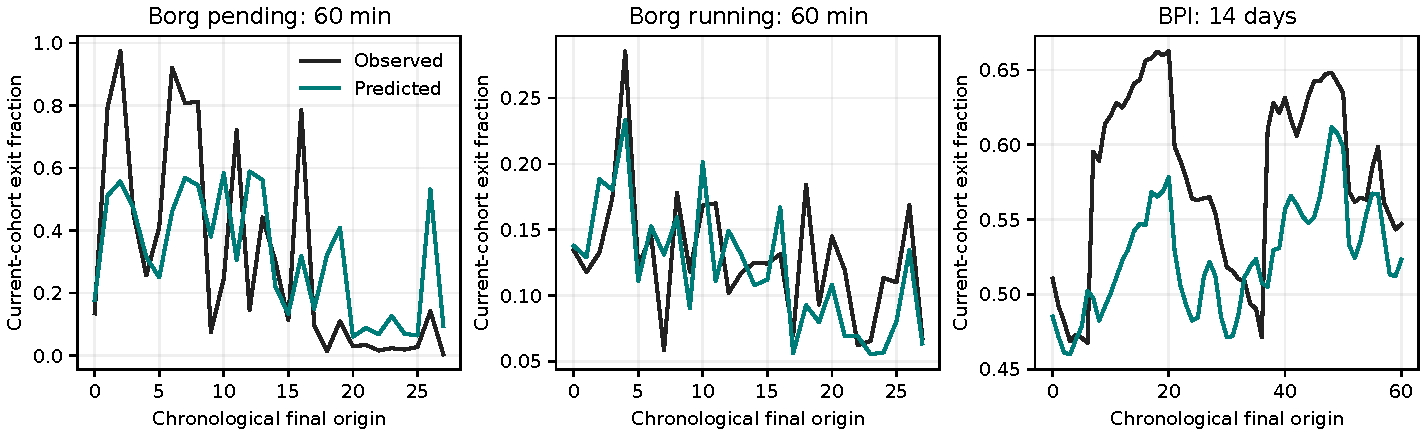
\includegraphics[width=\textwidth]{figures/marginal_bias.pdf}
\caption{Longest-horizon population mean forecasts and outcomes at each final
origin. These means are identical in expectation for all matched-marginal
dependence models. A copula changes dispersion and tails, but cannot repair
their mean forecast bias.}
\label{fig:bias}
\end{figure*}
\subsection{Marginal diagnostics and data-quality strata}
Figure~\ref{fig:bias} shows that dependence comparisons inherit distinct
marginal errors. At 60 minutes, mean Borg pending-task exit probability is
0.3193 versus an observed fraction of 0.3184. For running tasks the corresponding
values are 0.1199 and 0.1287. Their final integrated Brier scores are 0.08251
and 0.02937. The BPI 14-day bias is larger in absolute fraction, as discussed
above. A small pooled mean error is not evidence of conditional calibration at
every origin or relation group; the released reliability and origin tables
retain this variation.

Cutoff-defined strata also matter. About 21,876 running tasks per final origin
have unknown initial state age. Their integrated Brier is 0.00025, compared
with 0.03529 for known-age running tasks. Long-lived initial-state entities are
thus a relatively easy subpopulation, and pooled scores conceal that
heterogeneity. The unknown-age pending stratum contains only one task per
origin and cannot support a general robustness claim. Running tasks with a
known preceding publisher-imputed event have Brier 0.01078 versus 0.03006
without one; these are descriptive case-mix differences, not causal effects
of imputation. All strata remain in the primary complete-cohort evaluation.

\subsection{Numerical sensitivity and execution}
Doubling seed-0 scenario draws from 512 to 1,024 changes macro CRPS by at
most 0.000122 across the two applications, families, and five controls.
Within each application and family, the ordering of the five controls is
unchanged. This checks the reported CRPS comparisons against finite-ensemble
variation; it does not replace uncertainty over future forecast origins.

On the shared RTX A6000 host, each 512-draw Borg evaluation of all five
controls across 28 origins takes 245.8--251.0
seconds wall time, including sampling and scoring. The corresponding BPI
evaluation across 61 origins takes 3.48--3.68
seconds. Borg peak allocated PyTorch memory is at most 0.67\,GiB
per evaluation process and peak host resident memory is 2.05\,GiB.
These are evaluation costs with individual CDFs already computed, measured
while other evaluations share the device; they exclude data reconstruction,
training, and individual-model inference. They are not an isolated latency
benchmark.

The final artifact audit verifies all 264 frozen
file hashes, every final CDF and label trajectory, the exact frozen feature
transform, and the expected origins and comparisons. No frozen model or
evaluation file was modified during final evaluation. The separately audited
lossless timestamp correction is described in the appendix.


